\section{Monday, July 28}


\begin{center}
    {\Large \textbf{Generalization of NLP Models}}
    
    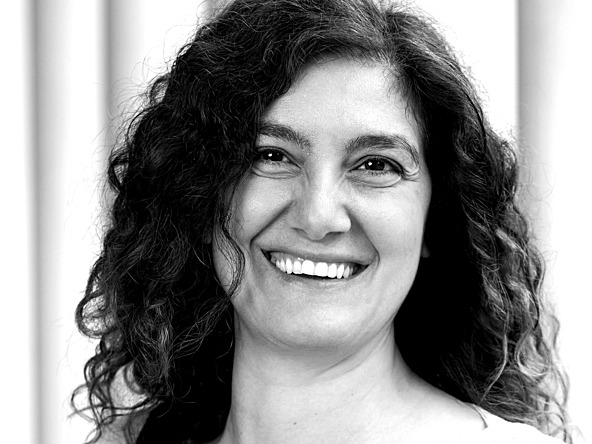
\includegraphics[width=1.5in]{examples/acl25-handbook/invited_talks/Mirella.jpg}
    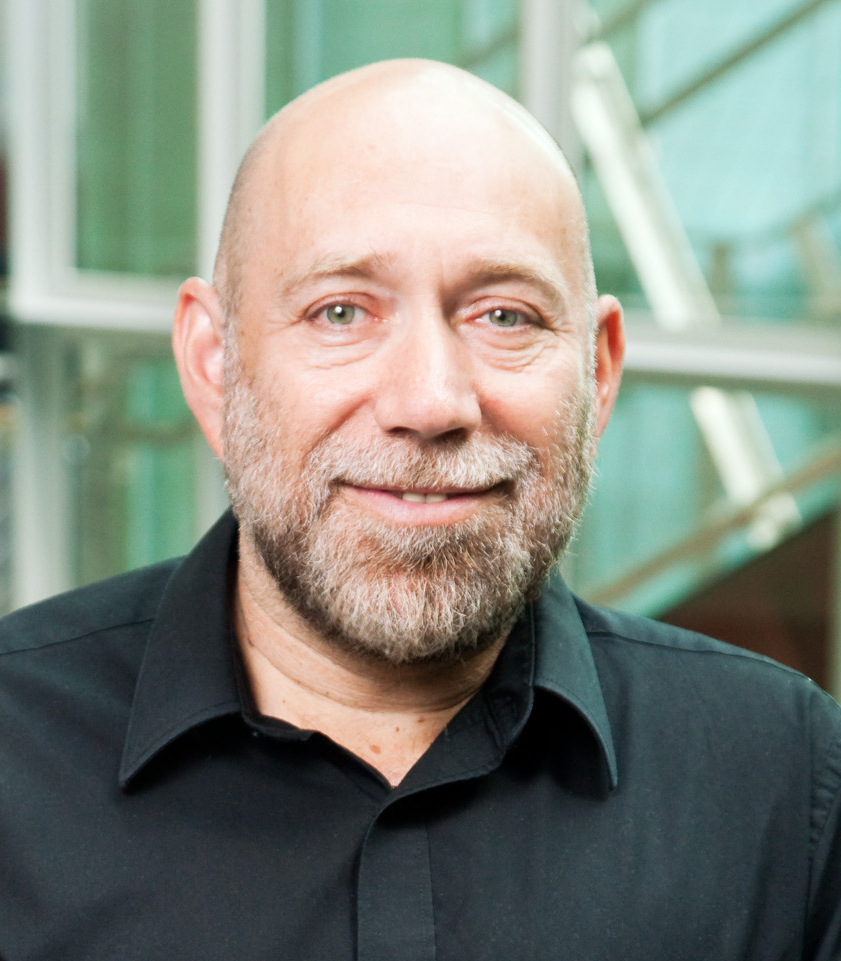
\includegraphics[width=1.5in]{examples/acl25-handbook/invited_talks/dan.jpg}
    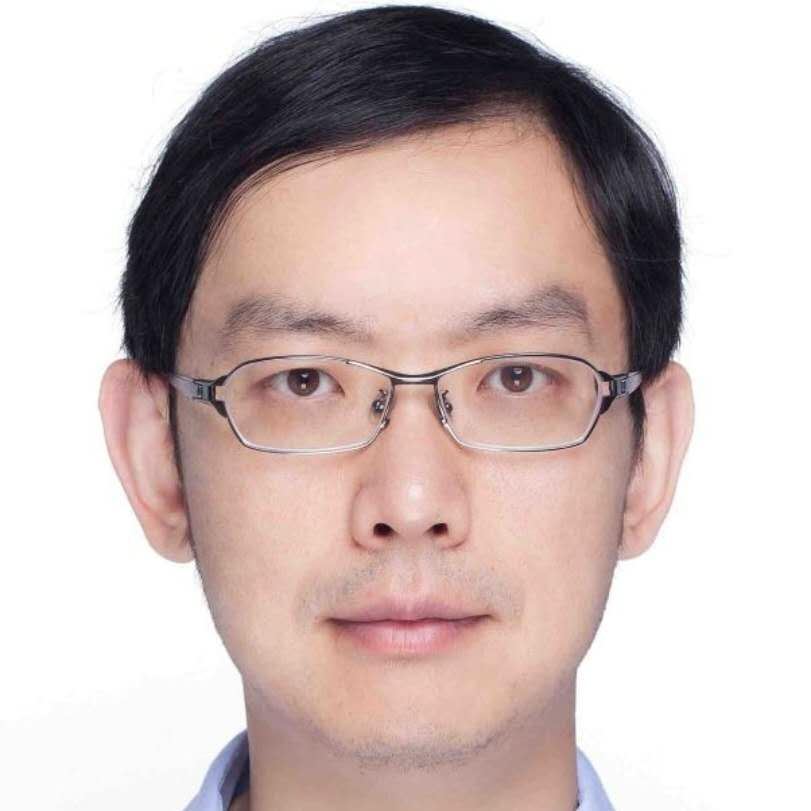
\includegraphics[width=1.5in]{examples/acl25-handbook/invited_talks/Yue.jpg}
    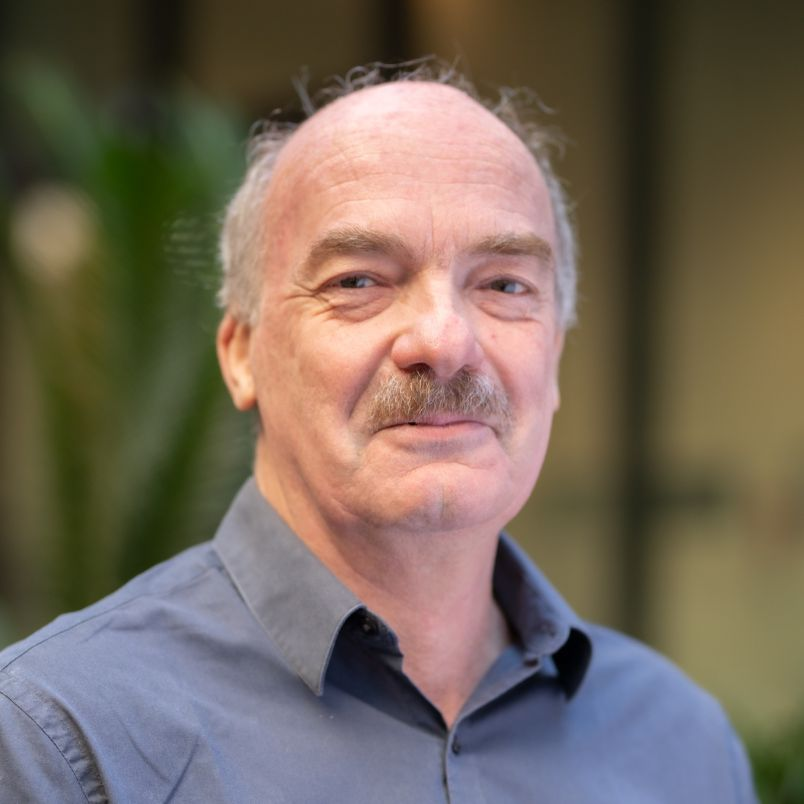
\includegraphics[width=1.5in]{examples/acl25-handbook/invited_talks/Ed.png}
    
    {\large \textbf{Panel: Mirella Lapata, Dan Roth, Yue Zhang}}\\
    {\large \textbf{Moderator: Eduard Hovy}}

    Monday, July 28, 16:30 - 17:30
\end{center}

\paragraph{Abstract:}
Large language model training follows a standard pipeline: tokenization, pretraining, possibly mid-training, and post training or alignment. Despite its wild success, we understand relatively little about this recipe and are almost certainly missing many opportunities to improve it. In this talk, I will focus on three such cases. I’ll describe our work on data efficient post training (e.g. LIMA, ALMA, and s1) where we argue that nearly all advanced model capabilities ultimately come from the pretraining data, even if effective alignment is still essential for controlling model behavior. I will also describe new methods for extracting more signal from the pretraining data, including new hierarchical architectures for byte-level language models (e.g. BLT) that are both tokenizer-free and scale better than traditional BPE-based methods, especially in the long tail. Finally, I will discuss decentralized, modular training algorithms (e.g. BTM) that better isolate and control the influence of specific data on specific model components and behaviors. Together, these methods promise to simplify training and improve scaling, by centering and amplifying the influence of data in architecture design. 

\paragraph{Bio:}
\textbf{Mirella Lapata} is professor of natural language processing in the School of Informatics at the University of Edinburgh. Her research focuses on getting computers to understand, reason with, and generate natural language. She is the first recipient (2009) of the British Computer Society and Information Retrieval Specialist Group (BCS/IRSG) Karen Sparck Jones award and a Fellow of the Royal Society of Edinburgh, the ACL, and Academia Europaea. Mirella has also received best paper awards in leading NLP conferences and has served on the editorial boards of the Journal of Artificial Intelligence Research, the Transactions of the ACL, and Computational Linguistics. She was president of SIGDAT (the group that organizes EMNLP) in 2018. She has been awarded an ERC consolidator grant, a Royal Society Wolfson Research Merit Award, and a UKRI Turing AI World-Leading Researcher Fellowship.\\

\textbf{Dan Roth} is the Eduardo D. Glandt Distinguished Professor at the University of Pennsylvania and Chief AI Scientist at Oracle. Until June 2024 Dan was a VP/Distinguished Scientist at AWS AI where he led the scientific effort behind Amazon’s first-generation GenAI products, including Titan Models, Amazon Q, and Amazon Bedrock.  Dan is a Fellow of the AAAS, ACM, AAAI, and ACL, and a recipient of the IJCAI John McCarthy Award “for major conceptual and theoretical advances in the modeling of natural language understanding, machine learning, and reasoning.” He has published broadly in natural language processing, machine learning, knowledge representation and reasoning, and learning theory, was the Editor-in-Chief of the Journal of Artificial Intelligence Research (JAIR) and has served as a Program Chair and Conference Chair for the major conferences in his research areas. Roth has been involved in several ML/NLP/GenAI startups in domains that range from legal and compliance to health care. Dan received his B.A Summa cum laude in Mathematics from the Technion, Israel and his Ph.D. in Computer Science from Harvard University in 1995.\\

\textbf{Yue Zhang} is a tenured Professor at Westlake University (https://frcchang.github.io). His research interests include fundamental NLP and its machine learning algorithms, and his recent research focuses on LLM reasoning and AI scientist. His major contributions to the field include machine learning algorithms for structured prediction (e.g., parsing and IE), neural NLP models (i.e., lattice and graph LSTM), and generalization for NLP/LM (e.g., OOD and logical reasoning). He co-authored the Cambridge University Press book ``Natural Language Processing -- a Machine Learning Perspective'‘ and served as a PC co-chair for CCL 2020 and EMNLP 2022, test-of-time award committee co-chairs for ACL 2024 and 2025, action editor for TACL, and associate editor for TASLP, TALLIP, TBD, and CSL. He won the best paper awards of IALP 2017 and COLING 2018, best paper honorable mention of SemEval 2020, and best paper nomination for ACL 2018 and ACL 2023.\\

\textbf{Eduard Hovy} is the Executive Director of Melbourne Connect (a research and tech transfer centre at the University of Melbourne), a professor at the University of Melbourne’s School of Computing and Information Systems, and an adjunct professor at the Language Technologies Institute in the School of Computer Science at Carnegie Mellon University.  In 2020–21 he served as Program Manager in DARPA’s Information Innovation Office (I2O), where he managed programs in Natural Language Technology and Data Analytics.  Dr. Hovy completed a Ph.D. in Computer Science (Artificial Intelligence) at Yale University in 1987 and was awarded honorary doctorates from the National Distance Education University (UNED) in Madrid in 2013 and the University of Antwerp in 2015.  He is one of the initial 17 Fellows of the Association for Computational Linguistics (ACL) and is also a Fellow of the Association for the Advancement of Artificial Intelligence (AAAI). Dr. Hovy’s research focuses on computational semantics of language and addresses various areas in Natural Language Processing and Data Analytics, including in-depth machine reading of text, information extraction, automated text summarization, question answering, the semi-automated construction of large lexicons and ontologies, and machine translation.  In early 2025 his Google h-index was 109, with about 68,000 citations. Dr. Hovy is the author or co-editor of eight books and over 400 technical articles and is a popular invited speaker.  He regularly co-taught Ph.D.-level courses and has served on Advisory and Review Boards for both research institutes and funding organizations in Germany, Italy, Netherlands, Ireland, Singapore, and the USA. From 2003 to 2015 he was co-Director of Research for the Department of Homeland Security’s Center of Excellence for Command, Control, and Interoperability Data Analytics, a distributed cooperation of 17 universities.  In 2001 Dr. Hovy served as President of the international Association of Computational Linguistics (ACL), in 2001–03 as President of the International Association of Machine Translation (IAMT), and in 2010–11 as President of the Digital Government Society (DGS).  


\index{panel}

\clearpage
